%!TEX root = ../main.tex
%=========================================================

\section{Ads placement}
\label{sec:placement}
In the following, we describe distributing advertisements in the network and discuss the process of search and establishing sub-protocol connections. We start by discussing the challenges related to the problem and explaining the data structures used by \sysname. 

\subsection{Challenges}
The first challenge of a robust service discovery platform is the question of where to store the advertisements. In other words, which nodes (registrars) in the network should be responsible for storing ads for each topic? It is possible to deterministically choose a group of nodes based on the topic itself using DHT put and get operations. Such a solution makes it \emph{efficient} to place and retrieve ads, as both advertisers and searchers know how to find common registrars and can reach them within a logarithmic amount of steps. Unfortunately, such an approach causes \emph{unequal} load distribution across registrars, especially when the popularity of the topics varies significantly. In particular, the registrars storing popular topics (\ie the ones closest to the hash of the popular topics) would receive a large portion of the registration requests in the network. Finally, this solution is \emph{not secure}, as an attacker could generate and strategically place its Sybil identities taking control over the entire topic-specific traffic. 

Alternatively, advertisers could place their ads on random registrars across the entire network. This approach is \emph{secure} and difficult to attack as an attacker would need to take control over the entire network to control a single topic. Furthermore, random placement is \emph{fair} and achieves good load balance across registrars regardless of the topic popularity distribution. However, random placement is not \emph{efficient}, as it makes it difficult for searchers to find placed ads, especially for unpopular topics. 

\sysname implements an alternative method of placing ads combining both the deterministic and pseudo-random approaches. Advertisers start the registration process from nodes located far away from the topic hash and traverse the DHT towards nodes close to the topic hash. On their way, advertisers place ads on encountered registrars with an increasing density. So that the closer to the topic hash, the higher number of ads are placed. The searchers mimic the process and ask encountered registrars for topic-specific ads. The lookup process stop, when enough ads are found.

\subsection{Data Structures}\label{sec:struct}
\sysname uses two data structures necessary for topic-specific registrations and lookups. 

\para{Advertise Table}
To execute the ad distribution process described below, each advertiser maintains an \emph{advertise table} for each advertised topic. The table keeps track of the ongoing registration attempts with different registrars. The \emph{advertise table} is similar to the routing table used in Kademlia protocol (as described in \Cref{sec:background}). It stores the advertiser's peers divided into k-buckets. However, instead of placing nodes in buckets based on the distance from the advertiser, it uses the distance from the topic ID. \Ie the \emph{advertise table} stores $K_\textit{register}$ potential registrars for every distance (bucket) from the topic ID (\Cref{fig:advertise_table}). When created, the table is initialized with peers from the routing table. 

\begin{figure}
    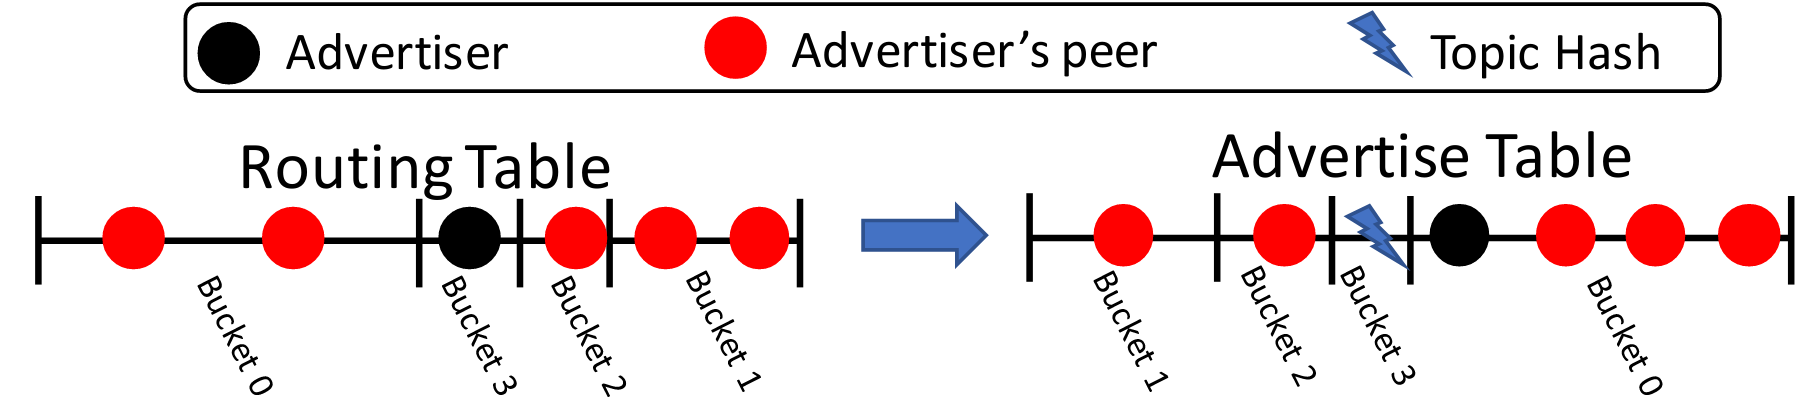
\includegraphics[width=0.45\textwidth]{img/tables}
    \caption{Creation of an advertise table from a routing table.} %\mk{To be reworked and make it consistent with other figures. E.g., we shouldn't use a circle to represent the hash space. We can maybe also try to illustrate here the mechanism of placing a fixed amount of ads in each bucket.}}
    \label{fig:advertise_table}
 \end{figure}

\para{Search Table}
The ad lookup process is supported by a \emph{search table}. 
Searchers maintain a separate table per topic they are currently looking for (\ie for each topic the client wants to start discovering nodes, a new \emph{search table} is created). 
Similar to the \emph{advertise table}, the \emph{search table} also stores k-buckets of registrar nodes by distance to the topic hash and buckets are initially filled from the local routing table organized by the distance from the topic hash.
\emph{Search table} buckets are also filled with new nodes discovered during the registration process.
%The \emph{k} factor of the search table should be relatively large to make the search efficient. 


\subsection{Distributing ads across registrars}\label{sec:registration_multi}
When an advertiser associates themselves with a topic, they start by creating a topic-specific \emph{advertise table} (as described above). 
Every peer present in the \emph{advertise table} is a potential registrar. 
The objective of the ad placement process is to continuously maintain $K_\textit{register}$ active (\ie unexpired) registrations in every bucket. 
Buckets located close to the topic hash cover less hash space than buckets located further away and, in turn, contain fewer potential registrars. 
Placing a fixed amount of ads per bucket, make registrars close to a topic hash more likely to receive registrations for that specific topic. 
Increasing $K_\textit{register}$, makes the advertiser easier to find at the cost of increased communication overhead. %More formally, the probability that a registrar has a topic-specific ad, based on the number of the nodes in a bucket $N_\textit{nodes}$, and the number of advertisers $N_\textit{advertisers}$ is given by:

%\begin{equation}
%   P_\textit{have ad} = 1-(1 - \frac{K_\textit{register}}{N_\textit{nodes}})^{N_\textit{advertisers}}
%\end{equation}
%\michal{TODO: Need to decide what to do with the equation above.}

For every bucket in the \emph{advertise table}, the advertiser selects
$K_{register}$ random peers and attempts to perform registration.
We describe details of the admission procedure in \Cref{sec:admission}. 
A successful registration places an ad on an advertiser for a fixed amount of time $a$.
If registration is unsuccessful (the selected registrar is down or refuses to store the ad), the advertiser selects another random peer from the same bucket and retries the registration process. 
The advertisers always maintain $K_\textit{register}$ attempts and/or
successful registrations per bucket unless there are less than $K_\textit{register}$ peers present in a specific bucket.
The advertiser repeats the process for every bucket in the \emph{advertise table}. 

The \emph{advertise table} is initialized with the peers already present in the routing table. It is thus possible that an advertiser will not know any nodes in buckets located close to the topic hash\footnote{This usually happens when the advertiser's ID is distant from the topic hash.}. 
To fill the empty buckets, the advertiser asks potential registrars to return $N$ closest peers to the topic hash they know of. 
The procedure is similar to the regular DHT \emph{FIND\_NODE} operation described in \Cref{sec:background}. 
The registrars respond with a list of peers regardless of the success of the registration operation. 
The advertiser uses the returned information to populate its \emph{advertise table}. 
As the advertiser progresses through the buckets, it queries potential registrars located closer to the topic hash and thus gets a more detailed view of this part of the network. 
Similar to the DHT routing, the registration procedure is guaranteed to find the closest node to the topic hash in the network within $O(log(N))$ number of steps. 

\subsection{Lookup operation}\label{sec:lookup}
To find ads, \sysname uses a process similar to the registration procedure. 
%The goal is to find $N_\textit{lookup}$ node advertised with a specific topic. 
%Each lookup requires a topic-specific \emph{search table} initially populated with nodes from the \emph{routing table}. 
Each lookup requires a topic-specific \emph{search table} described in \Cref{sec:struct}
The searcher progressively moves through buckets (starting from the furthest away), randomly chooses $K_\textit{lookup}$ registrars per bucket and sends them parallel lookup requests. 
Once received results from the first $K_\textit{lookup}$ selected registrars, other $K_\textit{lookup}$ registrars are selected from the following bucket with a smaller distance to the topic id.
The queried nodes are removed from the bucket.
Searchers stop the lookup procedure when they discover $N_\textit{lookup}$ peers. This is likely to happen far before reaching registrars located near the topic hash, especially for popular topics. As a result, \sysname avoids hot spots in the network and ensures fair load distribution. 
In case all buckets have been queried without finding enough nodes, the lookup process continues starting with the furthest distance bucket again. 
Once the lookup process is completed, the nodes are returned to the application.

Since the furthest buckets are also the largest (\ie it contains 50\% of all the honest registrars), an attacker placing malicious registrars in those buckets would require significant resources to eclipse the procedure. 
Searchers progressively moving towards smaller buckets near the topic hash guarantees successful discovery even for unpopular topics.
Each queried registrar responds with a list of $N_\textit{return}$ topic-specific advertisers the registrar knows of. 
If the total number of topic-specific registrations in the table is larger then
$N_\textit{return}$, the registrar should return a random subset.
While both $N_\textit{return}$ and $N_\textit{lookup}$ are protocol parameters,
the number of ads returned by a single registrar must be lower than the total
number of ads searchers are aiming to find $N_\textit{return} <
N_\textit{lookup}$. This is to diversify the sources of ads received by the searcher. \Ie, a single malicious registrar is not able to stop an honest searcher from contacting other nodes.
%\sergi{And is possible also a good idea to use a $N_\textit{lookup}$ parameter that forces that results from multiple buckets are used}
There is a trade-off between overhead and security when choosing $N_\textit{return}$ and $N_\textit{lookup}$. 
By requiring a large number of total ads to stop the search
($N_\textit{lookup}$) compared with the ads returned by the registrar
$N_\textit{return}$ a higher diversity of data sources is achieved at the cost of contacting a large number of registrars. On the other hand, similar values of both $N_\textit{lookup}$ and $N_\textit{return}$ reduce the overhead but increase the danger of a searcher receiving ads uniquely from malicious nodes. Finally, low values of $N_\textit{lookup}$ stop the search operation early, before reaching registrars close to the topic hash, contributing to a more equal load spread.
%However, for security reasons it is always recommendable to use $L_\textit{lookup}$, $N_\textit{return}$ and $N_\textit{lookup}$ parameters to ensure that at least 3 different registrars are queried from 2 different distance buckets.
%In the evaluation in \cref{sec:eval},  we set $L_\textit{lookup}=1$, $N_\textit{return}=10$ and $N_\textit{lookup}=30$, to be able to get results from 3 different registrars from 3 different buckets.
%\sr{Future work: investigate the impact of search parameters}

%\michal{For security, highlight that we want to mix results from different buckets and from different registrars - this is very important for security}
%\michal{Consider renaming search/advertise tables into search/registration caches}
%\michal{From Felix: 1) how exactly we choose the registrars to ask 2) filling the search table as you go 3) how many queries per node, how do you combine the results 4) when do you stop}
%\ramin{In practice, is $N_\textit{lookup}$ a parameter that can be controlled? It sounds like something application-specific, e.g. for some applications, it might be enough for a searcher to just find one node to be able to use the application as intended. Search for 10 and choose one randomly from them?}
%\michal{That's a good point. Not sure if we should allow the application to control both $N_\textit{lookup}$ and $N_\textit{return}$. Or maybe fix a ration between both and automatically set $N_\textit{return}$ once $N_\textit{lookup}$ is chosen by the application.}
%\sergi{I think $N_\textit{return}$ should not be configurable since it is limited by the maximum number of nodes returned in a message which i think is 16.  I think $N_\textit{lookup}$ can be configurable, but never smaller than a value multiple of $N_\textit{return}$}

